\documentclass{beamer}
\usepackage[utf8]{inputenc}

\usetheme{Madrid}
\usecolortheme{default}
\usepackage{amsmath,amssymb,amsfonts,amsthm}
\usepackage{txfonts}
\usepackage{tkz-euclide}
\usepackage{listings}
\usepackage{adjustbox}
\usepackage{array}
\usepackage{tabularx}
\usepackage{gvv}
\usepackage{lmodern}
\usepackage{circuitikz}
\usepackage{tikz}
\usepackage{graphicx}

\setbeamertemplate{page number in head/foot}[totalframenumber]

\usepackage{tcolorbox}
\tcbuselibrary{minted,breakable,xparse,skins}

\definecolor{bg}{gray}{0.95}
\DeclareTCBListing{mintedbox}{O{}m!O{}}{%
breakable=true,
listing engine=minted,
listing only,
minted language=#2,
minted style=default,
minted options={%
linenos,
gobble=0,
breaklines=true,
breakafter=,,
fontsize=\small,
numbersep=8pt,
#1},
boxsep=0pt,
left skip=0pt,
right skip=0pt,
left=25pt,
right=0pt,
top=3pt,
bottom=3pt,
arc=5pt,
leftrule=0pt,
rightrule=0pt,
bottomrule=2pt,
toprule=2pt,
colback=bg,
colframe=orange!70,
enhanced,
overlay={%
\begin{tcbclipinterior}
\fill[orange!20!white] (frame.south west) rectangle ([xshift=20pt]frame.north west);
\end{tcbclipinterior}},
#3,
}
\lstset{
language=C,
basicstyle=\ttfamily\small,
keywordstyle=\color{blue},
stringstyle=\color{orange},
commentstyle=\color{green!60!black},
numbers=left,
numberstyle=\tiny\color{gray},
breaklines=true,
showstringspaces=false,
}

\title
{2.4.40}
\date{September 17, 2025}
\author
{EE25BTECH11043 - Nishid Khandagre}

\begin{document}

\frame{\titlepage}

\begin{frame}{Question}
Find the angle between the lines $-\sqrt{3}x + y - 5 = 0$ and $- x + \sqrt{3}y + 6 = 0$.
\end{frame}

\begin{frame}{Theoretical Solution}

Given lines:
\begin{align}
L_1: -\sqrt{3}x + y - 5 &= 0 \\
L_2: - x + \sqrt{3}y + 6 &= 0
\end{align}

The matrix form of a line can be written as \\ 
\begin{align}
\vec{n}^\top \vec{x} = c
\end{align}
Where $\vec{n}$ is the normal vector and $\vec{x} = \myvec{x \\ y}$ is the position vector.
\end{frame}

\begin{frame}{Theoretical Solution}

\begin{align}
L_1: \vec{n_1}^\top\vec{x}&=c_1\\
L_2: \vec{n_2}^\top\vec{x}&=c_2
\end{align}

Where $\vec{n_1}$ and $\vec{n_2}$ are the normal vectors to the lines $L_1$ and $L_2$ respectively.
\begin{align}
\vec{n_1} &= \myvec{-\sqrt{3} \\ 1} \\
\vec{n_2} &= \myvec{-1 \\ \sqrt{3}}
\end{align}
\end{frame}

\begin{frame}{Theoretical Solution}
The angle $\theta$ between the lines is the angle between their normal vectors.
\begin{align}
\cos \theta = \frac{\vec{n_1}^\top \vec{n_2}}{\norm{\vec{n_1}} \norm{\vec{n_2}}} \label{eq:equation}
\end{align}

\begin{align}
\vec{n_1}^\top \vec{n_2} &= \myvec{ -\sqrt{3} & 1 } \myvec{-1 \\ \sqrt{3}} \\
&= (-\sqrt{3})(-1) + (1)(\sqrt{3}) \\
&= 2\sqrt{3}
\end{align}
\end{frame}

\begin{frame}{Theoretical Solution}
\begin{align}
\norm{\vec{n_1}} &= \sqrt{\vec{n_1}^\top\vec{n_1}}\\
&= \sqrt{(-\sqrt{3})^2 + (1)^2} \\
&= \sqrt{4} \\
&= 2
\end{align}

\begin{align}
\norm{\vec{n_2}} &= \sqrt{\vec{n_2}^\top\vec{n_2}}\\
&= \sqrt{(-1)^2 + (\sqrt{3})^2} \\
&= \sqrt{4} \\
&= 2
\end{align}
\end{frame}

\begin{frame}{Theoretical Solution}
Now, substitute these values into the formula \eqref{eq:equation}
\begin{align}
\cos \theta &= \frac{2\sqrt{3}}{(2)(2)} \\
&= \frac{\sqrt{3}}{2}
\end{align}

\begin{align}
\theta &= \frac{\pi}{6} \text{ radians}
\end{align}
\end{frame}

\begin{frame}[fragile]
\frametitle{C Code}
\begin{lstlisting}
#include <stdio.h>
#include <math.h>

// Function to calculate the angle between two lines in degrees
// given their slopes m1 and m2
void findAngleBetweenLines(double m1, double m2, double *angle_degrees) {
    // Calculate the tangent of the angle
    double tan_theta = (m1 - m2) / (1 + m1 * m2);

    // Calculate the angle in radians using atan
    double angle_radians = atan(tan_theta);

    // Convert the angle from radians to degrees
    *angle_degrees = angle_radians * (180.0 / M_PI);
    
\end{lstlisting}
\end{frame}
\begin{frame}[fragile]
\frametitle{C Code }
\begin{lstlisting}
    // Ensure the angle is positive
    if (*angle_degrees < 0) {
        *angle_degrees += 180.0;
    }
}

int main() {
    double m1, m2;        // Slopes of the two lines
    double calculated_angle_degrees; // Variable to store the calculated angle


    \end{lstlisting}
\end{frame}
\begin{frame}[fragile]
\frametitle{C Code }
\begin{lstlisting}
   
    // Call the function to calculate the angle
    findAngleBetweenLines(m1, m2, &calculated_angle_degrees);
    
    return 0;
}
\end{lstlisting}
\end{frame}

\begin{frame}[fragile]
\frametitle{Python Code through shared output }

\begin{lstlisting}
import ctypes
import math
import matplotlib.pyplot as plt
import numpy as np

# Load the shared library
lib_angle = ctypes.CDLL("./code3.so") 

# Define the argument types and return type for the C function
lib_angle.findAngleBetweenLines.argtypes = [
    ctypes.c_double,  # m1
    ctypes.c_double,  # m2
    ctypes.POINTER(ctypes.c_double) # angle_degrees
]
lib_angle.findAngleBetweenLines.restype = None

# Line 1: y - sqrt(3)x - 5 = 0  =>  y = sqrt(3)x + 5
# Slope m1 = sqrt(3)
\end{lstlisting}
\end{frame}

\begin{frame}[fragile]
\frametitle{Python Code through shared output }

\begin{lstlisting}
m1_given = math.sqrt(3)

# Line 2: sqrt(3)y - x + 6 = 0  => sqrt(3)y = x - 6 => y = (1/sqrt(3))x - 6/sqrt(3)

# Slope m2 = 1 / math.sqrt(3)
m2_given = 1 / math.sqrt(3)

# Create a ctypes double to hold the result
angle_result = ctypes.c_double()

# Call the C function to find the angle
lib_angle.findAngleBetweenLines(
    m1_given, m2_given, ctypes.byref(angle_result)
)

angle_found = angle_result.value
\end{lstlisting}
\end{frame}

\begin{frame}[fragile]
\frametitle{Python Code through shared output }

\begin{lstlisting}
print(f"The angle between the lines is {angle_found:.2f} degrees")

# --- Plotting the lines ---
# Generate x values
x_vals = np.linspace(-10, 10, 400)

# Calculate y values for Line 1: y = sqrt(3)x + 5
y1_vals = m1_given * x_vals + 5

# Calculate y values for Line 2: y = (1/sqrt(3))x - 6/sqrt(3)
y2_vals = m2_given * x_vals - 6 / math.sqrt(3)

plt.figure(figsize=(10, 8))

# Plot Line 1
plt.plot(x_vals, y1_vals, label=f'Line 1: y - $\\sqrt{{3}}$x - 5 = 0 (m={m1_given:.2f})', color='blue')
\end{lstlisting}
\end{frame}

\begin{frame}[fragile]
\frametitle{Python Code through shared output }

\begin{lstlisting}
# Plot Line 2
plt.plot(x_vals, y2_vals, label=f'Line 2: $\\sqrt{{3}}$y - x + 6 = 0 (m={m2_given:.2f})', color='red')

# Find intersection point for plotting
# Intersection of y = m1*x + c1 and y = m2*x + c2
# m1*x + c1 = m2*x + c2  => x(m1 - m2) = c2 - c1
# x = (c2 - c1) / (m1 - m2)
c1 = 5
c2 = -6 / math.sqrt(3)
x_intersect = (c2 - c1) / (m1_given - m2_given)
y_intersect = m1_given * x_intersect + c1 # Using Line 1 equation to find y

plt.scatter(x_intersect, y_intersect, color='green', s=100, zorder=5, label='Intersection')
\end{lstlisting}
\end{frame}

\begin{frame}[fragile]
\frametitle{Python Code through shared output }

\begin{lstlisting}
plt.annotate(
    f'({x_intersect:.2f}, {y_intersect:.2f})',
    xy=(x_intersect, y_intersect),
    xytext=(x_intersect + 1, y_intersect + 1), # Offset text for better readability
    fontsize=10,
    color='black'
)


plt.xlabel('X-axis')
plt.ylabel('Y-axis')
plt.title(f'Lines and the Angle Between Them ({angle_found:.2f} degrees)')
\end{lstlisting}
\end{frame}

\begin{frame}[fragile]
\frametitle{Python Code through shared output }

\begin{lstlisting}
plt.axhline(0, color='black', linewidth=0.5)
plt.axvline(0, color='black', linewidth=0.5)
plt.grid(True)
plt.legend()
plt.ylim(-10, 10) # Adjust y-limits for better viewing
plt.xlim(-10, 10) # Adjust x-limits for better viewing
plt.gca().set_aspect('equal', adjustable='box')
plt.savefig("fig1.png") % Save the plot
plt.show()
\end{lstlisting}
\end{frame}

\begin{frame}[fragile]
\frametitle{Python Code: Direct}
\begin{lstlisting}[language=Python]
import numpy as np
import matplotlib.pyplot as plt

def find_angle_between_lines_and_plot():
    # Line 1: y - sqrt(3)x - 5 = 0 
    # Slope m1 = sqrt(3)
    m1 = np.sqrt(3)

    # Line 2: sqrt(3)y - x + 6 = 0  
    # Slope m2 = 1 / np.sqrt(3)
    m2 = 1 / np.sqrt(3)

    # Calculate the angle using the formula: tan(theta) = (m1 - m2) / (1 + m1 * m2)
    # We use arctan to get the angle in radians.
    # The result will be in the range [-pi/2, pi/2].
    angle_radians = np.arctan((m1 - m2) / (1 + m1 * m2))
\end{lstlisting}

\end{frame}
\begin{frame}[fragile]
\frametitle{Python Code : Direct}

\begin{lstlisting}
    # Convert the angle from radians to degrees
    angle_degrees = np.degrees(angle_radians)

    # The formula gives an angle between -90 and 90 degrees.
    # To get the acute angle between lines, we take the absolute value.
    angle_degrees = abs(angle_degrees)

    # If the angle is obtuse, we subtract it from 180 to get the acute angle.
    if angle_degrees > 90:
        angle_degrees = 180 - angle_degrees

    print(f"The angle between the lines is {angle_degrees:.2f} degrees")
\end{lstlisting}

\end{frame}
\begin{frame}[fragile]
\frametitle{Python Code : Direct}

\begin{lstlisting}
    # --- Plotting the lines ---

    plt.figure(figsize=(10, 8))

    # Generate x values
    x_vals = np.linspace(-10, 10, 400)

    # Calculate y values for Line 1: y = sqrt(3)x + 5
    y1_vals = m1 * x_vals + 5

    # Calculate y values for Line 2: y = (1/sqrt(3))x - 6/np.sqrt(3)
    y2_vals = m2 * x_vals - 6 / np.sqrt(3)

    # Plot Line 1
    plt.plot(x_vals, y1_vals, label=f'Line 1: y - $\\sqrt{{3}}$x - 5 = 0 (m={m1:.2f})', color='blue')
\end{lstlisting}

\end{frame}
\begin{frame}[fragile]
\frametitle{Python Code : Direct}

\begin{lstlisting}
    # Plot Line 2
    plt.plot(x_vals, y2_vals, label=f'Line 2: $\\sqrt{{3}}$y - x + 6 = 0 (m={m2:.2f})', color='red')

    # Find the intersection point for labeling and drawing the angle
    c1 = 5
    c2 = -6 / np.sqrt(3)
    
    # Check for parallel lines (m1 == m2) to avoid division by zero
    if abs(m1 - m2) > 1e-9: 
        x_intersect = (c2 - c1) / (m1 - m2)
        y_intersect = m1 * x_intersect + c1
        plt.scatter(x_intersect, y_intersect, color='green', s=100, zorder=5, label='Intersection Point')
        \end{lstlisting}

\end{frame}
\begin{frame}[fragile]
\frametitle{Python Code : Direct}

\begin{lstlisting}
        plt.annotate(f'({x_intersect:.2f}, {y_intersect:.2f})', 
                     (x_intersect, y_intersect), 
                     textcoords="offset points", xytext=(5,5), ha='left')
    else:
        print("The lines are parallel.")
        x_intersect = None
        y_intersect = None

    plt.xlabel('X-axis')
    plt.ylabel('Y-axis')
    plt.title(f'Lines and the Angle Between Them ({angle_degrees:.2f} degrees)')
    plt.axhline(0, color='black', linewidth=0.5)
    plt.axvline(0, color='black', linewidth=0.5)
    \end{lstlisting}

\end{frame}
\begin{frame}[fragile]
\frametitle{Python Code : Direct}

\begin{lstlisting}
    plt.grid(True)
    plt.legend()
    plt.ylim(-10, 10)
    plt.xlim(-10, 10)
    plt.gca().set_aspect('equal', adjustable='box')
    plt.savefig("fig2.png") % Save the plot
    plt.show()

    print("Figure saved as fig2.png")

# Call the function to execute the code and generate the plot
find_angle_between_lines_and_plot()
\end{lstlisting}
\end{frame}

\begin{frame}{Plot by Python using shared output from C}
\begin{figure}[H]
        \centering
        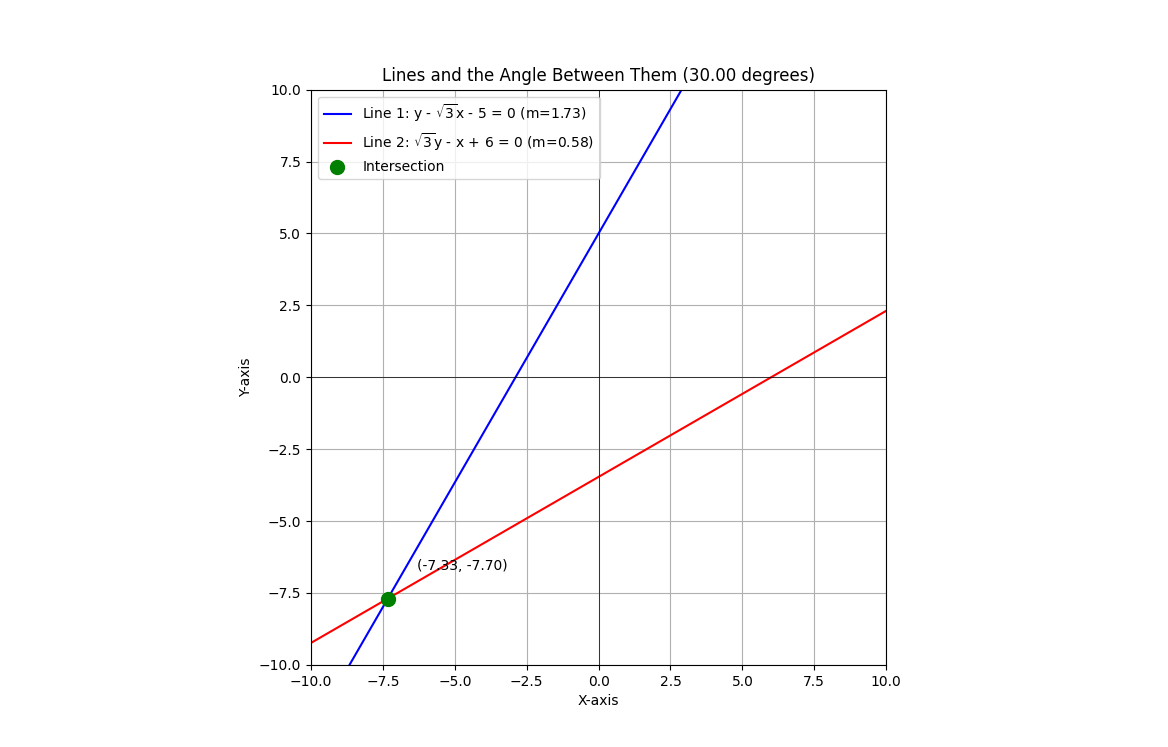
\includegraphics[width=1.0\columnwidth]{../figs/fig1.png}
        \caption{}
        \label{fig:1}
    \end{figure}
\end{frame}

 \begin{frame}{Plot by Python only}
\begin{figure}[H]
        \centering
        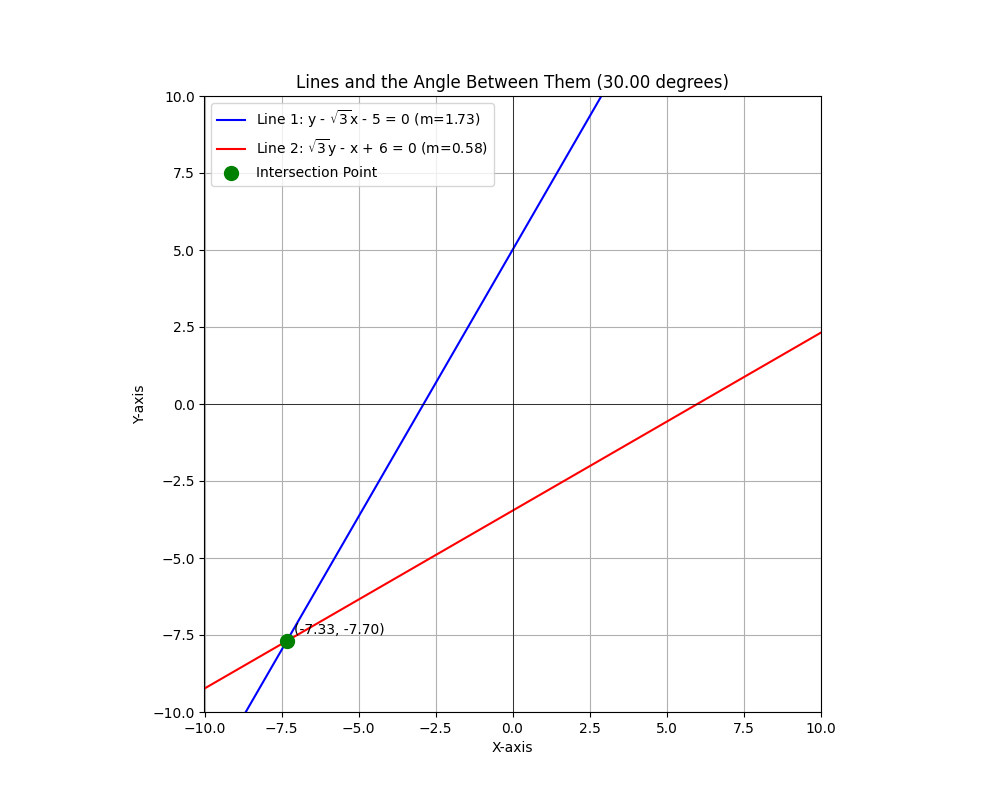
\includegraphics[width=0.8\columnwidth]{../figs/fig2.png}
        \caption{}
        \label{fig:2}
    \end{figure}
\end{frame}

\end{document}
